\chapter{METHODOLOGY}
\label{ch:methodology}

\section{Introduction}

This chapter defines the experimental design. It begins with the dataset, since its
size and structure constrain everything that follows. A sample of 11 annotated
images drawn from four specimens is small and strongly hierarchical, and the
evaluation protocol therefore has to be built around this fact rather than around
convention. Roberts et al.\ \cite{roberts2017crossvalidation} set out why data with
a hierarchical structure require the partition to respect that hierarchy, while
Kapoor and Narayanan \cite{kapoor2023leakage} document how frequently the omission
has produced published results that do not hold.
The chapter then describes the physical calibration that allows pixel measurements
to be reported in micrometres, the six methods under comparison, and the metrics.

\section{Research Design}

The study is experimental and comparative. Six methods drawn from four families,
namely a classical thresholding pipeline, a semantic encoder--decoder network, two
region-based detectors and two one-stage detectors, are applied to the same
images under an identical partitioning scheme, and are assessed both by
conventional segmentation metrics and by the counting and sizing errors that
determine whether the output is usable in the laboratory.

The comparison is structured so each method isolates one factor. The
classical pipeline establishes what is achievable without training data. The
semantic network establishes what is gained by learning while still producing only
a foreground mask. The region-based instance network adds explicit instance
separation, so the difference between the second and the third measures the value
of instance-level modelling rather than of deep learning in general. The remaining
methods vary one component at a time within this structure.

\section{Dataset}

\subsection{Acquisition and Structure}

The dataset consists of SEM images of electrospun nanofibre membranes, acquired on
a Zeiss instrument at an accelerating voltage of 15.00\,kV and at working
distances between 8.5 and 11.0\,mm. Every image is $1024 \times 768$ pixels,
8-bit greyscale, stored as JPEG.

The 11 images are not independent samples. They derive from four specimens,
denoted S1, S2, S3 and S4, each imaged at $500\times$, $1000\times$ and
$3000\times$. The numeric suffix in a filename encodes the magnification rather
than a repeat acquisition, so S1-1, S1-2 and S1-3 are three views of one specimen.
One combination is absent, as specimen S2 has no $500\times$ image, and
specimen S4 uses the identifier S4-4 for its $3000\times$ view. The four specimens
are four different production methods and not four repeats of one, which is what
makes the partitioning choice of Section~\ref{sec:protocol} consequential rather
than procedural: holding out a specimen holds out a production method, so a model
generalising across the folds has generalised across the process and not merely
across the frame.

\begin{table}[htbp]
    \centering

    \caption{The 11 annotated images. Specimen and magnification are recovered
    from the filename and confirmed against the instrument banner burned into each
    image. All images are $1024 \times 768$ px at 15.00\,kV.}
    \label{tab:dataset}
    \begin{tabular}{llrrrr}
        \toprule
        Image & Specimen & Mag. & WD (mm) & Beads & Median $d$ (px) \\
        \midrule
        S1-1 & S1 & $500\times$  & 10.0 & 71  & 14.2 \\
        S1-2 & S1 & $1000\times$ & 10.0 & 51  & 28.8 \\
        S1-3 & S1 & $3000\times$ & 10.0 & 10  & 76.3 \\
        \midrule
        S2-2 & S2 & $1000\times$ & 9.0  & 59  & 24.4 \\
        S2-3 & S2 & $3000\times$ & 9.0  & 4   & 68.0 \\
        \midrule
        S3-1 & S3 & $500\times$  & 8.5  & 102 & 12.9 \\
        S3-2 & S3 & $1000\times$ & 8.5  & 57  & 22.1 \\
        S3-3 & S3 & $3000\times$ & 8.5  & 14  & 53.9 \\
        \midrule
        S4-1 & S4 & $500\times$  & 11.0 & 152 & 15.7 \\
        S4-2 & S4 & $1000\times$ & 11.0 & 62  & 28.7 \\
        S4-4 & S4 & $3000\times$ & 11.0 & 24  & 75.4 \\
        \midrule
        \textbf{Total} & 4 specimens & 3 mags & & \textbf{606} & \\
        \bottomrule
    \end{tabular}
\end{table}

Figure~\ref{fig:dataset_overview} shows one specimen at all three magnifications
with its annotations overlaid. The change in apparent object size is the dominant
visual difference between the three panels, and it is the reason why a scale-robust
model is required.

\begin{figure}[htbp]
    \centering
    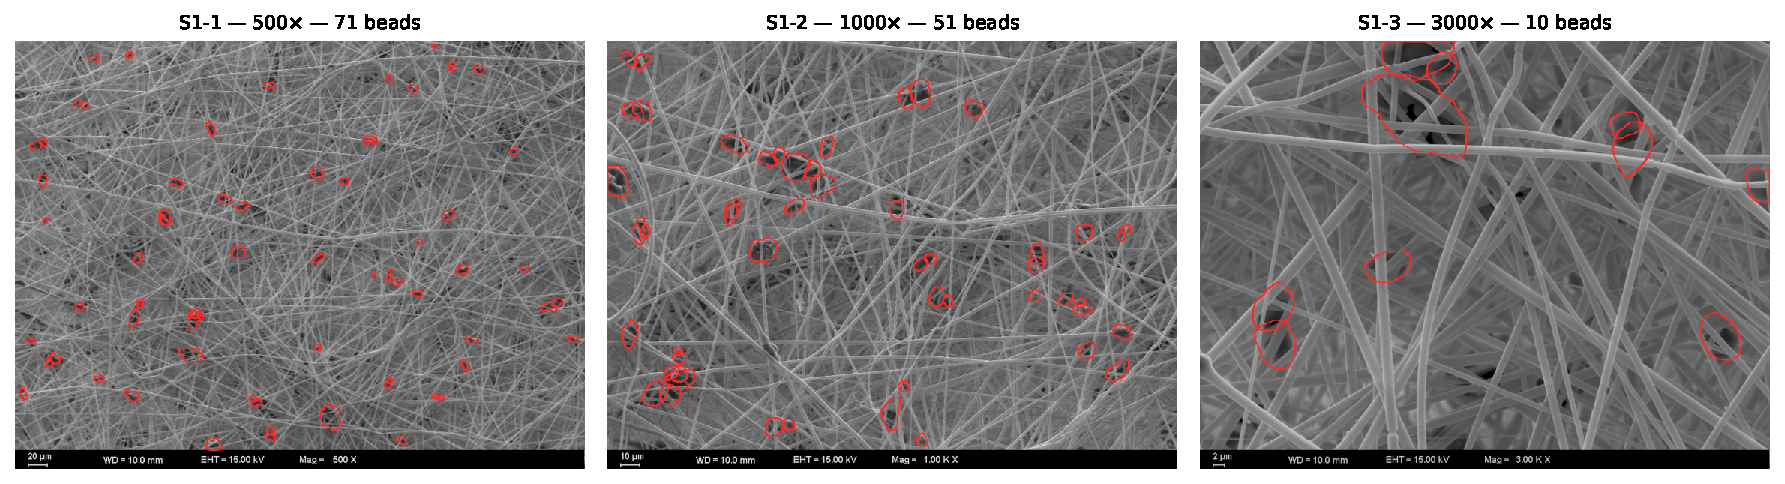
\includegraphics[width=\textwidth]{figures/fig_dataset_overview.pdf}
    \caption{Specimen S1 imaged at $500\times$, $1000\times$ and $3000\times$, with
    the manual bead annotations overlaid in red. The same beads appear at roughly
    14, 29 and 76 pixels across, and the count within the field falls from 71 to 10
    as the field of view narrows.}
    \label{fig:dataset_overview}
\end{figure}

\subsection{Annotation}

The annotations were produced in LabelMe (version 5.4.1) and are supplied as one
JSON file per image. Every annotated object is a closed polygon carrying the
single class label \texttt{bead}, and the polygons contain between 8 and 40
vertices, with a median of 16. Across the 11 images there are 606 annotated
beads. No annotation intersects the instrument banner region described in
Section~\ref{sec:banner}.

The dataset is therefore single-class, as the task is to separate beads from
everything else and no distinction is drawn between bead subtypes.

\subsubsection{What Counts as an Object}
\label{sec:object_definition}

A segmentation result is interpretable only against a definition of the thing
being segmented, so the three rules to which the annotator worked are stated here
rather than left implicit in the polygons. They were specified by the supervisor,
who directs the group that produced the specimens.

The first rule is circularity. The embedded zeolite particles, referred to
throughout this thesis as beads since the two terms denote the same objects, are
approximately circular in projection, so an object is annotated when it presents
as a compact, roughly circular body, and not when it presents as an elongated
fibre segment.

The second is that swellings count. Where a fibre thickens locally into such a
body, that swelling is annotated as a bead even though the fibre passes through
it. In these images this is the common case rather than the exception, which is
why no distinction is drawn between a free bead and a thickened fibre segment.

The third is that a cluster is one object. Where several small beads lie together,
the group is outlined once rather than resolved into its members.

The third rule carries a consequence Chapter~\ref{ch:results} has to live with. A
method that splits a cluster into its visible members is scored as having made a
split error, even where its output may be closer to the number of individual
crystals present. What is counted here is therefore bead sites, and the merge
and split rates of Section~\ref{sec:comparison} measure agreement with that
convention rather than with crystal-level truth; the distinction is revisited
among the limitations in Section~\ref{sec:limitations}.

Two properties of the annotation constrain the implementation and are shown in
Figures~\ref{fig:bead_examples} and \ref{fig:overlap}. The same physical object is
presented at very different resolutions, as the median bead of specimen S4
measures about 8\,$\mu$m at every magnification while spanning 16 pixels at
$500\times$ and 77 at $3000\times$. And beads touch: 8.8\% of annotated bead
pixels lie inside more than one polygon, so the annotation is not a partition of
the image and cannot be stored as one without discarding exactly the regions where
merge and split errors are decided.

\begin{figure}[htbp]
    \centering
    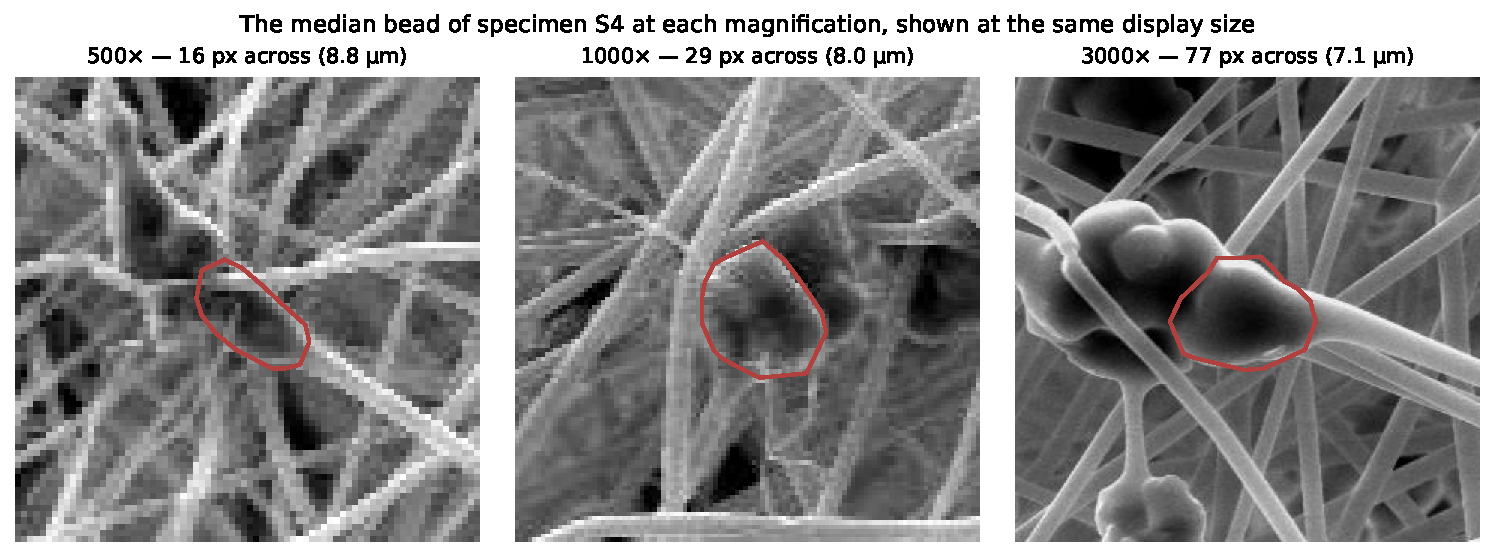
\includegraphics[width=\textwidth]{figures/fig_bead_examples.pdf}
    \caption{The median bead of specimen S4 at each magnification, each crop
    scaled to the same display size. The physical diameter is nearly constant
    while the pixel diameter varies almost fivefold.}
    \label{fig:bead_examples}
\end{figure}

\begin{figure}[htbp]
    \centering
    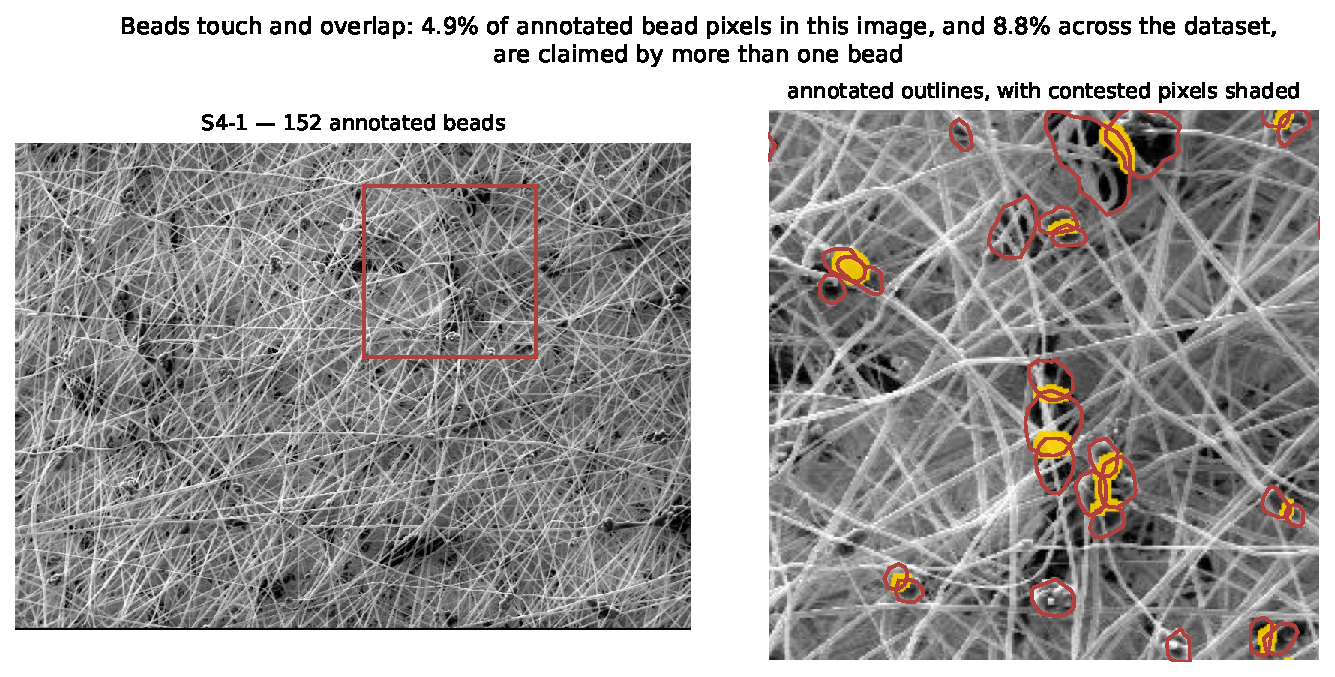
\includegraphics[width=\textwidth]{figures/fig_overlap.pdf}
    \caption{A region of S4-1 in which annotated beads share pixels. Red outlines
    are the manual annotation and shaded pixels are claimed by more than one
    bead.}
    \label{fig:overlap}
\end{figure}

\subsection{Physical Calibration}
\label{sec:calibration}

Each image carries a burned-in scale bar. Measuring the bar in pixels and
dividing by its stated physical length yields the pixel size, and the values
recovered in this way are mutually consistent, since the field width is
$284.4\,\mu$m at $1000\times$ and scales inversely with magnification, as it must.
The resulting calibration is given in Table~\ref{tab:calibration}.

\begin{table}[htbp]
    \centering
    \caption{Pixel size recovered from the burned-in scale bars. The field width is
    inversely proportional to magnification, confirming that the three values form a
    consistent calibration rather than three independent measurements.}
    \label{tab:calibration}
    \begin{tabular}{lrrr}
        \toprule
        Magnification & Field width ($\mu$m) & Pixel size (nm/px) & Beads \\
        \midrule
        $500\times$  & 568.9 & 555.6 & 325 \\
        $1000\times$ & 284.4 & 277.8 & 229 \\
        $3000\times$ & 94.8  & 92.6  & 52  \\
        \bottomrule
    \end{tabular}
\end{table}

Bead size is expressed as an equivalent circular diameter, that is the diameter of
the circle having the same area as the outlined bead. The area is computed
analytically from the polygon vertices $(x_1, y_1), \dots, (x_N, y_N)$ by the
shoelace formula, with indices taken modulo $N$,
%
\begin{equation}
    A = \frac{1}{2}
        \left| \sum_{i=1}^{N} \bigl( x_i \, y_{i+1} - x_{i+1} \, y_i \bigr) \right|,
    \label{eq:shoelace}
\end{equation}
%
rather than by counting the pixels of a rasterised mask. The distinction is not
pedantic in this case, since at $500\times$ the median bead is only about 14 pixels
across, so a one-pixel error along its boundary changes the area by roughly
15\%. The equivalent diameter in micrometres then follows from the pixel size $s$ of
Table~\ref{tab:calibration},
%
\begin{equation}
    d = 2 s \sqrt{\frac{A}{\pi}}.
    \label{eq:equivalent_diameter}
\end{equation}

The calibration can be validated independently of the scale bars. If it is correct,
the physical bead size distribution measured at one magnification should agree with
that measured at another, since all three views image the same specimens. Grouping
every annotated polygon by magnification gives median diameters of 7.92, 7.34 and 6.75\,$\mu$m at $500\times$,
$1000\times$ and $3000\times$ respectively, which is agreement to within 15\%. This
satisfies the criterion set in Section~\ref{sec:objectives} and confirms both the
calibration and the internal consistency of the annotation. The three distributions
are compared in Figure~\ref{fig:bead_statistics}.

\begin{figure}[htbp]
    \centering
    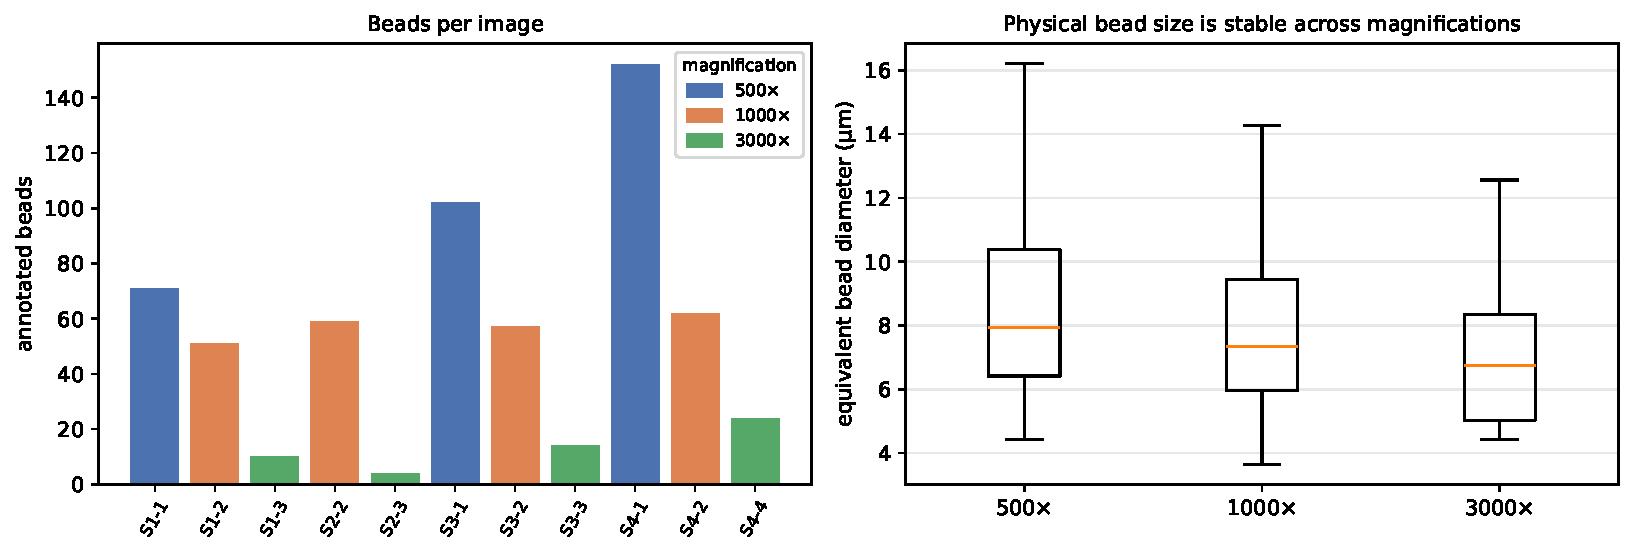
\includegraphics[width=\textwidth]{figures/fig_bead_statistics.pdf}
    \caption{Left: annotated beads per image, coloured by magnification; the
    $3000\times$ images contribute only 52 of the 606 annotated beads. Right:
    equivalent bead diameter in micrometres, grouped by magnification. The three
    distributions overlap, as they must if the calibration is correct.}
    \label{fig:bead_statistics}
\end{figure}

The residual downward trend with magnification, from 7.92 to 6.75\,$\mu$m, is
consistent with a sampling effect rather than a calibration error. At $3000\times$
the field is only 94.8\,$\mu$m wide, so a large bead is more likely to be clipped
by the image border and excluded, and only 52 beads are observed in total.

\subsection{The Instrument Banner}
\label{sec:banner}

Every image carries a burned-in information banner occupying the bottom 32
pixels, containing the scale bar, working distance, accelerating voltage and
magnification. The banner is not part of the specimen: it is high-contrast,
identical in structure across images, and correlates with magnification, so a
network trained on uncropped images could read the magnification off the banner
instead of learning scale-invariant features. It is therefore cropped before any
processing, leaving an effective image size of $1024 \times 736$. No annotation is
lost, since no annotated polygon extends into the banner region, and the
calibration values of Table~\ref{tab:calibration} are extracted once before
cropping and carried forward as metadata.

\subsection{The Supplied Augmentations}
\label{sec:supplied_aug}

The dataset as received contains 143 image--annotation pairs rather than 11. Each
of the 11 originals is accompanied by 12 pre-computed augmented copies: a
horizontal flip, a vertical flip, eight translations of $\pm 150$ pixels along
each axis and in combination, and two horizontal stretches of 20\% and 40\%. The
polygon coordinates were transformed along with the images and remain correctly
registered in every variant.

These copies are nevertheless excluded, for three reasons. The first is
statistical: thirteen copies of one image contain the information of one
image, so reporting 143 images, or 7\,878 bead instances, would misstate the
sample size by a factor of 13.

\begin{figure}[htbp]
    \centering
    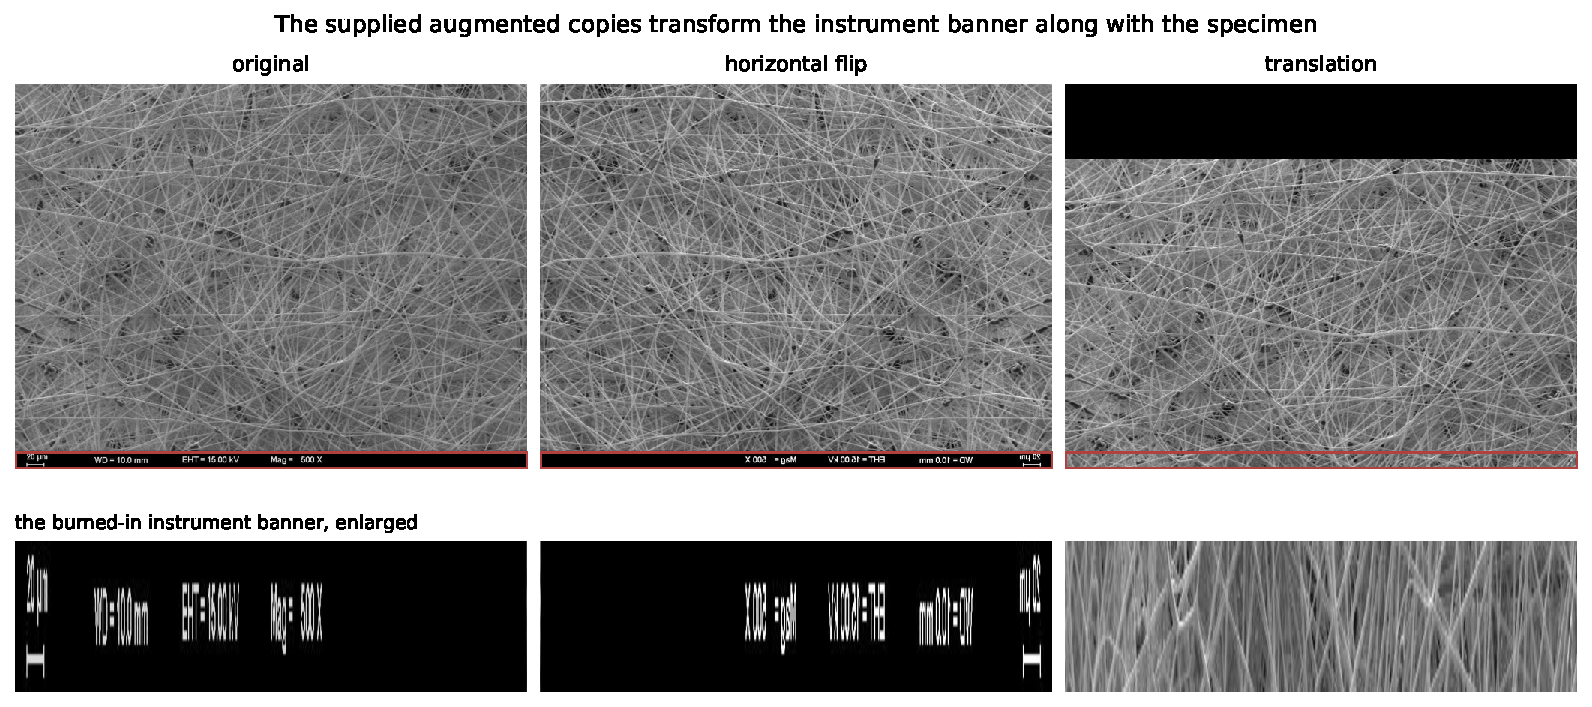
\includegraphics[width=\textwidth]{figures/fig_augmentation_problem.pdf}

    \caption{Three of the 143 supplied files: one original and two of its
    pre-computed augmented copies, with the instrument banner outlined and
    enlarged beneath each. The flip mirrors the burned-in text and the translation
    leaves black fill along the top edge.}
    \label{fig:augmentation_problem}
\end{figure}

The second reason is methodological and more serious. Since the copies were
generated before partitioning, a random split over the 143 files would place
transformed versions of the same source image in both the training and the
test partition, and the test score would then partly measure memorisation.
Augmentation is still used, as it is essential at this sample size, but applied on
the fly during training, after partitioning, so no test image has a transformed
relative in the training set.

The third is visible in Figure~\ref{fig:augmentation_problem}: the transformations
were applied to the whole file, including the instrument banner. The flipped
copies carry mirrored burned-in text and the translated copies carry black fill
along the vacated edge, so the copies are not merely redundant but carry an
artefact a network can key on.

\section{Evaluation Protocol}
\label{sec:protocol}

The four specimens, and not the eleven images, are the independent units of
this dataset. Images S1-1, S1-2 and S1-3 are three views of the same physical
material, sharing its polymer, its spinning parameters and its particular
population of beads, so a partition placing S1-1 in training and S1-3 in testing
measures generalisation to a new magnification of a specimen already seen rather
than to a new specimen.

\begin{figure}[htbp]
    \centering
    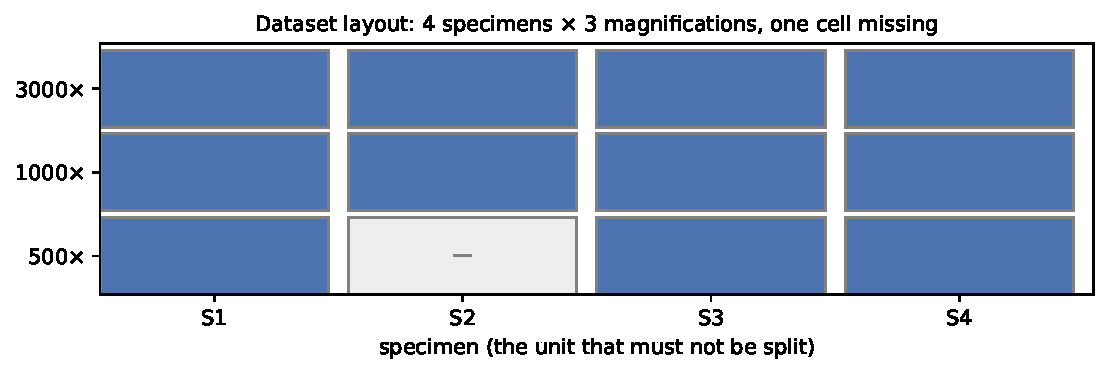
\includegraphics[width=0.75\textwidth]{figures/fig_split_protocol.pdf}
    \caption{Layout of the dataset. Each column is a specimen and each row a
    magnification, and the shaded cells are the 11 available images. Specimen
    S2 has no $500\times$ image.}
    \label{fig:split_protocol}
\end{figure}

The protocol adopted is therefore \emph{leave-one-specimen-out
cross-validation}. Each of the four folds trains on all images of three
specimens and tests on all images of the fourth, so every image is used
for testing exactly once and no specimen is ever split. Results are reported as
the mean over folds together with the spread, which at this sample size is itself
an important number.

To quantify what this protocol costs, and therefore what a naive protocol would
have overstated, a second and deliberately flawed configuration is also run, in
which the 11 images are split at random without regard to specimen. The
difference is reported in Chapter~\ref{ch:results}, and this comparison is one of
the stated contributions of the thesis, since it converts a methodological
argument into a measured quantity.

\section{Methods}

\subsection{Classical Baseline: Otsu Thresholding with Watershed}

The classical pipeline represents current laboratory practice. The cropped
image is contrast-normalised, thresholded with Otsu's method
\cite{otsu1979threshold} and cleaned with morphological opening and closing, and
the resulting binary mask is split into instances by a watershed transform
\cite{vincent1991watersheds} applied to its distance transform with local maxima
as markers. Components smaller than a minimum area, expressed in physical units
through the calibration of Section~\ref{sec:calibration}, are discarded. The
baseline requires no training data, so it is evaluated on all 11 images
directly, with its parameters tuned once on the training folds and held fixed.

\subsection{Semantic Baseline: U-Net}

The semantic baseline is a U-Net \cite{ronneberger2015unet} with a ResNet encoder
\cite{he2016deep} initialised from ImageNet weights \cite{deng2009imagenet},
trained to predict a binary bead-versus-background mask, with instances recovered
afterwards by connected-component labelling. It is included specifically to
isolate the cost of merging: it is expected to segment bead pixels well while
merging clusters of touching beads into single components, and the gap between its
pixel-level and its count-level performance is the quantity of interest.

\subsection{Instance Segmentation: Mask R-CNN}

The primary model is Mask R-CNN \cite{he2017mask} with a ResNet-50 backbone
\cite{he2016deep} and a feature pyramid network \cite{lin2017feature}, initialised
from COCO-pretrained weights \cite{lin2014microsoft}. The region proposal network
proposes candidate boxes, and for each surviving proposal the network predicts a
class, a refined box and a binary mask within the region, so touching beads are
separated by construction. The feature pyramid assigns proposals to levels
according to their size, which is the mechanism by which a single model can handle
beads spanning 14 to 76 pixels across. Anchor scales are set from the empirical
bead size distribution rather than left at their COCO defaults, since the median
bead occupies 0.04\% of the image area.

\subsection{Detection Without Segmentation: Faster R-CNN}

The endpoint this work exists to serve is a count, and a count requires only
detection. Faster R-CNN \cite{ren2015faster} is therefore included as a controlled
ablation of the mask branch of Mask R-CNN: the two share the ResNet-50 and feature
pyramid backbone, the anchor sizes, the cap on detections, the optimiser, the
schedule, the fold definitions and the rule fixing the score threshold on each
fold's training partition. The mask branch is the only difference, so a gap
between them is attributable to it. The same architecture was applied to counting
cells in low-contrast images by Uka et al.\ \cite{uka2020faster}.

Its predictions are stored as boxes with no segmentation field, so it is absent
from every mask-level result: the Aggregated Jaccard Index, Panoptic Quality, the
merge and split rates and the size distribution are mask quantities, and filling
each box to manufacture one would score the method on something it never
predicted. What the ablation can compare is the count, defined identically for
both.

\subsection{One-Stage Alternatives: YOLOv8 and YOLOv5u}

YOLOv8 \cite{redmon2016yolo, jocher2023ultralytics} is the one-stage family of
Section~\ref{sec:onestage}, included to answer a different question from the
ablation above, namely whether a different family of architecture performs better
on this data. It is not a controlled comparison and is not read as one, since it
shares nothing with the region-based models, having a different backbone, an
anchor-free head, a different label assignment rule, a different loss and its own
augmentation and optimiser schedule, so a gap between it and Mask R-CNN identifies
no component as responsible. The segmentation variant is used, so it predicts
masks and is scored on every metric the region-based instance model is.

YOLOv5u is included alongside it, sharing the Ultralytics training loop, the same
three departures from its defaults and the same number of training iterations, while differing
in the backbone and in carrying no mask branch, since the package ships no
segmentation weights for YOLOv5. Two models rather than one make the family
comparison less dependent on a single checkpoint.

The checkpoint is \texttt{yolov5su}, the YOLOv5 backbone fitted by Ultralytics
with the anchor-free, objectness-free split head of YOLOv8, and not the
anchor-based YOLOv5 of the original release. What separates it from
\texttt{yolov8s-seg} is therefore mostly the backbone and the mask branch. The
results are labelled YOLOv5u throughout.

Three settings depart from the package defaults, each for a measured property of
this dataset rather than by search. The input size is held at 1024 rather than the
default 640, since downscaling a $1024 \times 736$ image by 0.625 would take
the median bead at $500\times$ from 14.3 to 8.9 pixels. Mosaic augmentation is
disabled, because composing four images and rescaling roughly halves the apparent
object size while 82.8\% of the beads are already below the small-object
threshold of COCO. Each model is likewise allowed to return up to 400 objects from one
image, since a single image here can hold 152 annotated beads and the default
would discard real detections without reporting that it had.

One consequence has to be stated with the results. The data pipeline of the
package expects a fixed directory of images rather than the crops the region-based
models draw on demand, so both YOLO models train on whole images at 1024
pixels while the region-based models train on $512 \times 512$ crops. Their
training cost is therefore not comparable with that of the region-based models.

\subsection{Preprocessing as an Experimental Factor}
\label{sec:preprocessing_method}

Prior work from this institution reports that the preprocessing applied before a
network sees an image changes materially what it can learn, for images
suffering from non-uniform illumination and low contrast
\cite{uka2020preprocessing}. The present dataset shares the low contrast, with
about eighteen grey levels separating a bead from the surrounding membrane, but
differs in one respect that governs which transforms are worth testing: in
unstained brightfield the background is a smooth field, whereas here it is a dense
fibre network with structure at the same spatial scale as the beads. The
transforms are therefore selected for this material rather than carried across.

Four variants are compared, with the architecture, schedule, fold definitions and
threshold-selection rule held fixed, so any difference is attributable to the
input transform alone:

The first variant applies no transform at all, and it is not merely a formality.
Both detectors are initialised from weights trained on natural images, which carry
expectations about intensity statistics, so a transform can as easily cost
accuracy as buy it, and a variant that loses to this baseline is a finding.

The second is CLAHE, contrast-limited adaptive histogram equalisation, applied
against the narrow separation. It is adaptive rather than global because the
brightness of the membrane varies across a frame by more than the
bead-to-membrane difference.

The third is background subtraction. The beads are darker than the membrane, so
the illumination estimate is a grey closing, which erases dark features while
preserving the slowly varying field. Its footprint has to exceed the largest
object present, and since the largest annotated bead spans 214 pixels the
footprint is set to 257.

The fourth is a median filter, a $3\times3$ median against sensor noise, kept
deliberately small since the median bead is 20 pixels across and a window
approaching that size would remove the object along with the noise.

Each variant is applied to the whole image before cropping, at the single
point where the training and inference paths share code. This is a correctness
requirement rather than a convenience, since a model trained on equalised images
and evaluated on raw ones would still produce numbers, wrong in a way no metric
would reveal.

\section{Evaluation Metrics}

\subsection{Segmentation and Detection Metrics}

Throughout this section, $G = \{g_1, \dots, g_n\}$ denotes the set of annotated bead
masks in an image and $P = \{p_1, \dots, p_m\}$ the set of predicted masks, with
$|\cdot|$ the area of a mask in pixels. The overlap between two masks is measured by
the intersection over union,
%
\begin{equation}
    \mathrm{IoU}(g, p) = \frac{|g \cap p|}{|g \cup p|}.
    \label{eq:iou}
\end{equation}

Detection and mask quality are reported as average precision at an
intersection-over-union threshold of 0.5 ($\mathrm{AP}_{50}$), at 0.75
($\mathrm{AP}_{75}$), and averaged over thresholds from 0.5 to 0.95 following the
COCO protocol \cite{lin2014microsoft}. Average precision at a fixed overlap
threshold originates with the Pascal VOC challenge \cite{everingham2010pascal},
while the COCO variant averages over a range of thresholds so boundary accuracy is
rewarded rather than only detection.

The aggregated Jaccard index \cite{kumar2017dataset} is reported in addition,
since it penalises merges and splits explicitly rather than treating each object
independently. Each annotated bead $g_i$ is assigned the prediction it overlaps
most,
%

\begin{equation}
    j^{*}(i) = \arg\max_{j} \; \mathrm{IoU}(g_i, p_j),
    \label{eq:aji_match}
\end{equation}
%
and writing $M$ for the beads whose best overlap is non-zero, $\bar{M}$ for those
with none, and $U$ for the predictions never selected by any bead,
%
\begin{equation}
    \mathrm{AJI} =
    \frac{\displaystyle\sum_{i \in M} \bigl|g_i \cap p_{j^{*}(i)}\bigr|}
         {\displaystyle\sum_{i \in M} \bigl|g_i \cup p_{j^{*}(i)}\bigr|
          \;+\; \sum_{i \in \bar{M}} |g_i|
          \;+\; \sum_{k \in U} |p_k|}.
    \label{eq:aji}
\end{equation}

%
Every predicted object that matches nothing, and every bead matched by nothing,
therefore enters the denominator and lowers the score, which is what makes the
index sensitive to over-segmentation where a per-object average is not.

Panoptic quality \cite{kirillov2019panoptic} is reported to separate
recognition from delineation. A predicted and an annotated mask are matched when
$\mathrm{IoU}(g, p) > 0.5$, and since no mask can exceed that overlap with more than
one partner, the matching is unique and requires no assignment solver. Writing
$\mathit{TP}$ for the matched pairs and $\mathit{FP}$, $\mathit{FN}$ for the
unmatched predictions and beads,
%
\begin{equation}
    \mathrm{PQ} =
    \underbrace{\frac{\sum_{(g,p) \in \mathit{TP}} \mathrm{IoU}(g,p)}
                     {|\mathit{TP}|}}_{\textstyle \mathrm{SQ}}
    \times
    \underbrace{\frac{|\mathit{TP}|}
                     {|\mathit{TP}| + \tfrac{1}{2}|\mathit{FP}|
                      + \tfrac{1}{2}|\mathit{FN}|}}_{\textstyle \mathrm{RQ}}.
    \label{eq:pq}
\end{equation}

%
The two factors are reported separately as well as combined, since they answer
different questions: segmentation quality $\mathrm{SQ}$ measures how well the
beads that are found are outlined, whereas recognition quality $\mathrm{RQ}$
measures how many were found at all. A method can be strong on one and weak on the
other, and Chapter~\ref{ch:results} shows the distinction matters here.

Finally, one measure deliberately discards instance identity. Flattening each side
to a single binary mask, $\hat{G} = \bigcup_i g_i$ and $\hat{P} = \bigcup_j p_j$,
gives the pixel-level agreement
%

\begin{equation}
    \mathrm{DICE} = \frac{2\,|\hat{G} \cap \hat{P}|}{|\hat{G}| + |\hat{P}|},
    \qquad
    \mathrm{IoU}_{\text{px}} = \frac{|\hat{G} \cap \hat{P}|}
                                    {|\hat{G} \cup \hat{P}|}.
    \label{eq:pixel_dice}
\end{equation}

%
This is the weakest measure in the chapter and is not used to rank anything, since
it cannot distinguish a method that separates two touching beads from one that
fuses them. It is reported for one reason: the semantic segmentation literature,
including the prior work of Section~\ref{sec:epoka_prior}, reports DICE and IoU
computed this way, and those values cannot be read against an average precision,
so computing both from the same predictions is what makes them comparable. The
counts are pooled over images before the ratio is formed, so a frame holding
four beads does not weigh as much as one holding 152.

\subsection{Laboratory Metrics}

Segmentation metrics do not by themselves establish that a method is usable, so
the following are reported as primary outcomes.

The counting error is the error in the number of beads found in an image,
as a fraction of the number actually present, reported both signed and absolute
since a method whose errors cancel behaves differently from one that is biased:
%

\begin{equation}
    e = 100 \times \frac{|G| - |P|}{|G|} \quad (\%),
    \label{eq:counting_error}
\end{equation}
%
positive for an under-count and negative for an over-count, with the sign written
out wherever the quantity appears.

The merge and split rates are the two failure modes that corrupt a
count, and since they have opposite effects on it they are reported separately.
Both are defined through the asymmetric coverage of one mask by another,
%
\begin{equation}
    c_{G}(g, p) = \frac{|g \cap p|}{|g|},
    \qquad
    c_{P}(g, p) = \frac{|g \cap p|}{|p|},
    \label{eq:coverage}
\end{equation}
%
with a threshold of $\tau = 0.5$ throughout. A prediction is a \emph{merge} when it
contains at least half of each of two or more annotated beads, and every bead that
it absorbed counts as merged, whereas an annotated bead is \emph{split} when it
contains at least half of each of two or more predictions:
%
\begin{align}
    \mathrm{merge\ rate} &= \frac{100}{|G|}
        \Bigl|\bigl\{\, g \in G \;:\; \exists\, p \in P,\;
        c_{G}(g,p) \geq \tau \;\wedge\;
        |\{g' \in G : c_{G}(g',p) \geq \tau\}| \geq 2 \,\bigr\}\Bigr|,
    \label{eq:merge_rate} \\[4pt]
    \mathrm{split\ rate} &= \frac{100}{|G|}
        \Bigl|\bigl\{\, g \in G \;:\;
        |\{p \in P : c_{P}(g,p) \geq \tau\}| \geq 2 \,\bigr\}\Bigr|.
    \label{eq:split_rate}
\end{align}

%
Coverage is used rather than intersection over union because the two failures are
asymmetric: a prediction swallowing two beads has a low $\mathrm{IoU}$ with each
while containing both almost entirely, so an overlap-based criterion would miss
exactly the case being measured.

Areal density is beads per square millimetre, the form in which the
measurement is used for process comparison. For an image of $W \times H$
pixels at a pixel size of $s$ micrometres,
%

\begin{equation}
    \rho = \frac{|P| \times 10^{6}}{W H s^{2}}
    \quad (\mathrm{beads\ mm^{-2}}).
    \label{eq:density}
\end{equation}

Size distribution agreement compares the predicted and the manual distributions of
equivalent bead diameter in micrometres, compared by their medians and interquartile
ranges and by a two-sample Kolmogorov--Smirnov test.

\section{Tools and Technologies}

The implementation uses Python with PyTorch. Annotations are parsed from the
LabelMe JSON format and converted to COCO-style instance masks, the classical
baseline uses scikit-image and OpenCV, and figures and statistics are produced
with Matplotlib and NumPy. Full version information is given in
Chapter~\ref{ch:implementation}. No local GPU was available, so the training
stages were run on Google Colab with an NVIDIA T4, with consequences for the
experimental design set out in Section~\ref{sec:environment}.

The dataset comprises 11 SEM images of four electrospun specimens, imaged at
three magnifications and annotated with 606 bead polygons. Each image is
calibrated against its burned-in scale bar, and the calibration is validated by
the agreement of the physical bead size distribution across magnifications. Since
the specimen is the only independent unit, evaluation uses leave-one-specimen-out
cross-validation, and the pre-computed augmented copies supplied with the dataset
are excluded in favour of augmentation applied after partitioning. Six methods,
namely classical thresholding, a semantic U-Net, Mask R-CNN, the same detector
without its mask branch, and the YOLOv8 and YOLOv5u one-stage models, are compared
under this protocol. The next chapter describes how the design is realised in
software.
